\documentclass[10pt,a4paper]{article}
\usepackage[margin=2.2cm]{geometry}
\usepackage[T1]{fontenc}
\usepackage[sc]{mathpazo}
\usepackage[scaled=.92]{helvet}
\usepackage{courier}
\linespread{1.05}
\usepackage{amsmath,amssymb}
\usepackage{siunitx}
\usepackage{graphicx}
\usepackage{booktabs,tabularx,array}
\usepackage{xcolor}
\usepackage{caption}
\usepackage{float}
\usepackage{enumitem}
\usepackage{listings}
\usepackage[hidelinks]{hyperref}
\graphicspath{{../build/fig/}}
\definecolor{accent}{HTML}{5B43A8}
\definecolor{gm}{HTML}{ECC6E3}
\definecolor{wm}{HTML}{7AA6DC}
\definecolor{codebg}{HTML}{F4F2EC}
\captionsetup{font=small,labelfont={bf,color=accent}}
\lstset{basicstyle=\ttfamily\small,backgroundcolor=\color{codebg},frame=none,columns=fullflexible,breaklines=true,
        keepspaces=true,xleftmargin=4pt,aboveskip=6pt,belowskip=6pt}
\setlist{itemsep=1pt,topsep=3pt}
\newcommand{\code}[1]{\texttt{#1}}
\newcommand{\step}[1]{\textbf{\color{accent}#1}}
% written by python -m medfig report; do not edit
\newcommand{\vExampleY}{-22}
\newcommand{\vRawW}{1970}
\newcommand{\vRawH}{1890}
\newcommand{\vDownW}{656}
\newcommand{\vDownH}{630}
\newcommand{\vNPlanes}{12}
\newcommand{\vTissueChanged}{290}
\newcommand{\vExOtsu}{198.5}
\newcommand{\vExThr}{194.5}
\newcommand{\vPtsRaw}{6373}
\newcommand{\vPtsSimple}{902}
\newcommand{\vVbW}{523}
\newcommand{\vVbH}{525}
\newcommand{\vMmPerUnit}{0.3}
\newcommand{\vDs}{3}
\newcommand{\vTBlur}{1.0}
\newcommand{\vTMax}{238}
\newcommand{\vTObj}{400}
\newcommand{\vTHole}{60}
\newcommand{\vLSig}{1.2}
\newcommand{\vFloor}{140}
\newcommand{\vOffset}{4}
\newcommand{\vRSig}{1.6}
\newcommand{\vWIsl}{120}
\newcommand{\vCSig}{1.6}
\newcommand{\vEps}{0.35}
\newcommand{\vPad}{24}
\newcommand{\vBlk}{82}
\newcommand{\vPersp}{1000}
\newcommand{\vTx}{38\%}
\newcommand{\vRy}{42}
\newcommand{\vRx}{6}
\newcommand{\vSc}{0.82}
\newcommand{\vDz}{95}
\newcommand{\vPhTx}{20\%}
\newcommand{\vPhRy}{46}
\newcommand{\vPhSc}{0.6}
\newcommand{\vPhDz}{55}
\newcommand{\vPhMax}{900}
\newcommand{\vZStart}{-420}
\newcommand{\SectionRows}{1 & $+8$ & frontal lobe and striatum & putamen & $(-24,\,4)$ & 190.9 & 197.3 & 193.3 \\
2 & $-22$ & thalamus and hippocampus & hippocampus & $(-27,\,-14)$ & 197.2 & 198.5 & 194.5 \\
3 & $-64$ & occipital lobe and cerebellum & cerebellar hemisphere & $(-26,\,-40)$ & 137.9 & 191.4 & 187.4 \\}
\newcommand{\SectionDelays}{0.00 & 0.12 & 0.26}
\newcommand{\MarkerDelays}{0.35 & 0.62 & 0.76}
\newcommand{\SvgSizes}{section\_1.svg: 47.1 KB, section\_2.svg: 49.7 KB, section\_3.svg: 55.7 KB}


\title{\textbf{medfig}: flat coronal brain figures from BigBrain\\and an oblique 3D section stack\\[4pt]
\large Methods report and reproduction guide}
\author{Kolachalama Laboratory, Boston University\\\small Prepared with Claude for the neuropathology VLM demo}
\date{13 October 2026 \quad$\cdot$\quad medfig 0.1.0}

\begin{document}
\maketitle

\begin{abstract}
\noindent
This report describes \textbf{medfig}, a small pipeline that turns the BigBrain \SI{100}{\micro\metre} histological volume into flat,
publication-style figures of coronal brain sections, and that animates three such sections as an oblique 3D stack in a web page.
The pipeline reads whole coronal planes out of the 1.1~GB compressed volume without loading it, separates grey from white matter
with a per-section threshold, converts the masks into smoothed vector outlines, places every section in one shared frame with
anatomically placed block markers, and derives slide icons whose tissue matches each block. Every step is a Python module, every
parameter is in one JSON file, and every number quoted below is written by the pipeline itself (\code{report/numbers.tex}).
The figures are a schematic: they do not show the Boston University cutting plan or BU block locations.
\end{abstract}

\section{Purpose and scope}
The landing page of the lab's neuropathology vision-language-model demo shows how the model is asked about one slide
(\emph{slide level}) or about all slides of a case (\emph{case level}). The illustration needs (i) a coronal section with one
sampled block, and (ii) for the case level, several sections of one brain, each with its own block, in a view that reads as 3D
and that switches smoothly from (i). An earlier version reused one drawn section three times, so the three sections looked the same.
medfig replaces it with real anatomy: three different coronal planes of one brain, drawn in the flat style of the page.

\paragraph{Out of scope.} medfig does not reproduce a stain (BigBrain uses a Merker cell-body stain, not H\&E or LFB-H\&E),
does not register to BU material, and makes no quantitative claim about any region.

\section{Data}
\textbf{BigBrain} \cite{amunts2013} is a 3D reconstruction of one human brain from 7404 Merker-stained sections.
medfig uses the release in ICBM2009b symmetric space \cite{fonov2011} at \SI{100}{\micro\metre}, 8-bit
(\nolinkurl{full8_100um_2009b_sym.nii.gz}, $1970\times2330\times1890$ voxels, 1.1~GB compressed, about 8.7~GB raw).
The repository holds \nolinkurl{data/bigbrain_coronal_100um_sel.npz} (10~MB): \vNPlanes{} whole coronal planes from
$y=+24$ to $-72$~mm cut from that volume (Section~\ref{s:s1}). The licence is CC~BY-NC-SA~4.0; every derived SVG carries the credit
in a comment and is shared under the same licence.

In Merker stain, cell bodies are dark. Grey matter is therefore \emph{darker} than white matter, the cerebellar granular layer is
nearly black, and glass is white (255).

\section{Pipeline overview}
\begin{figure}[H]
\centering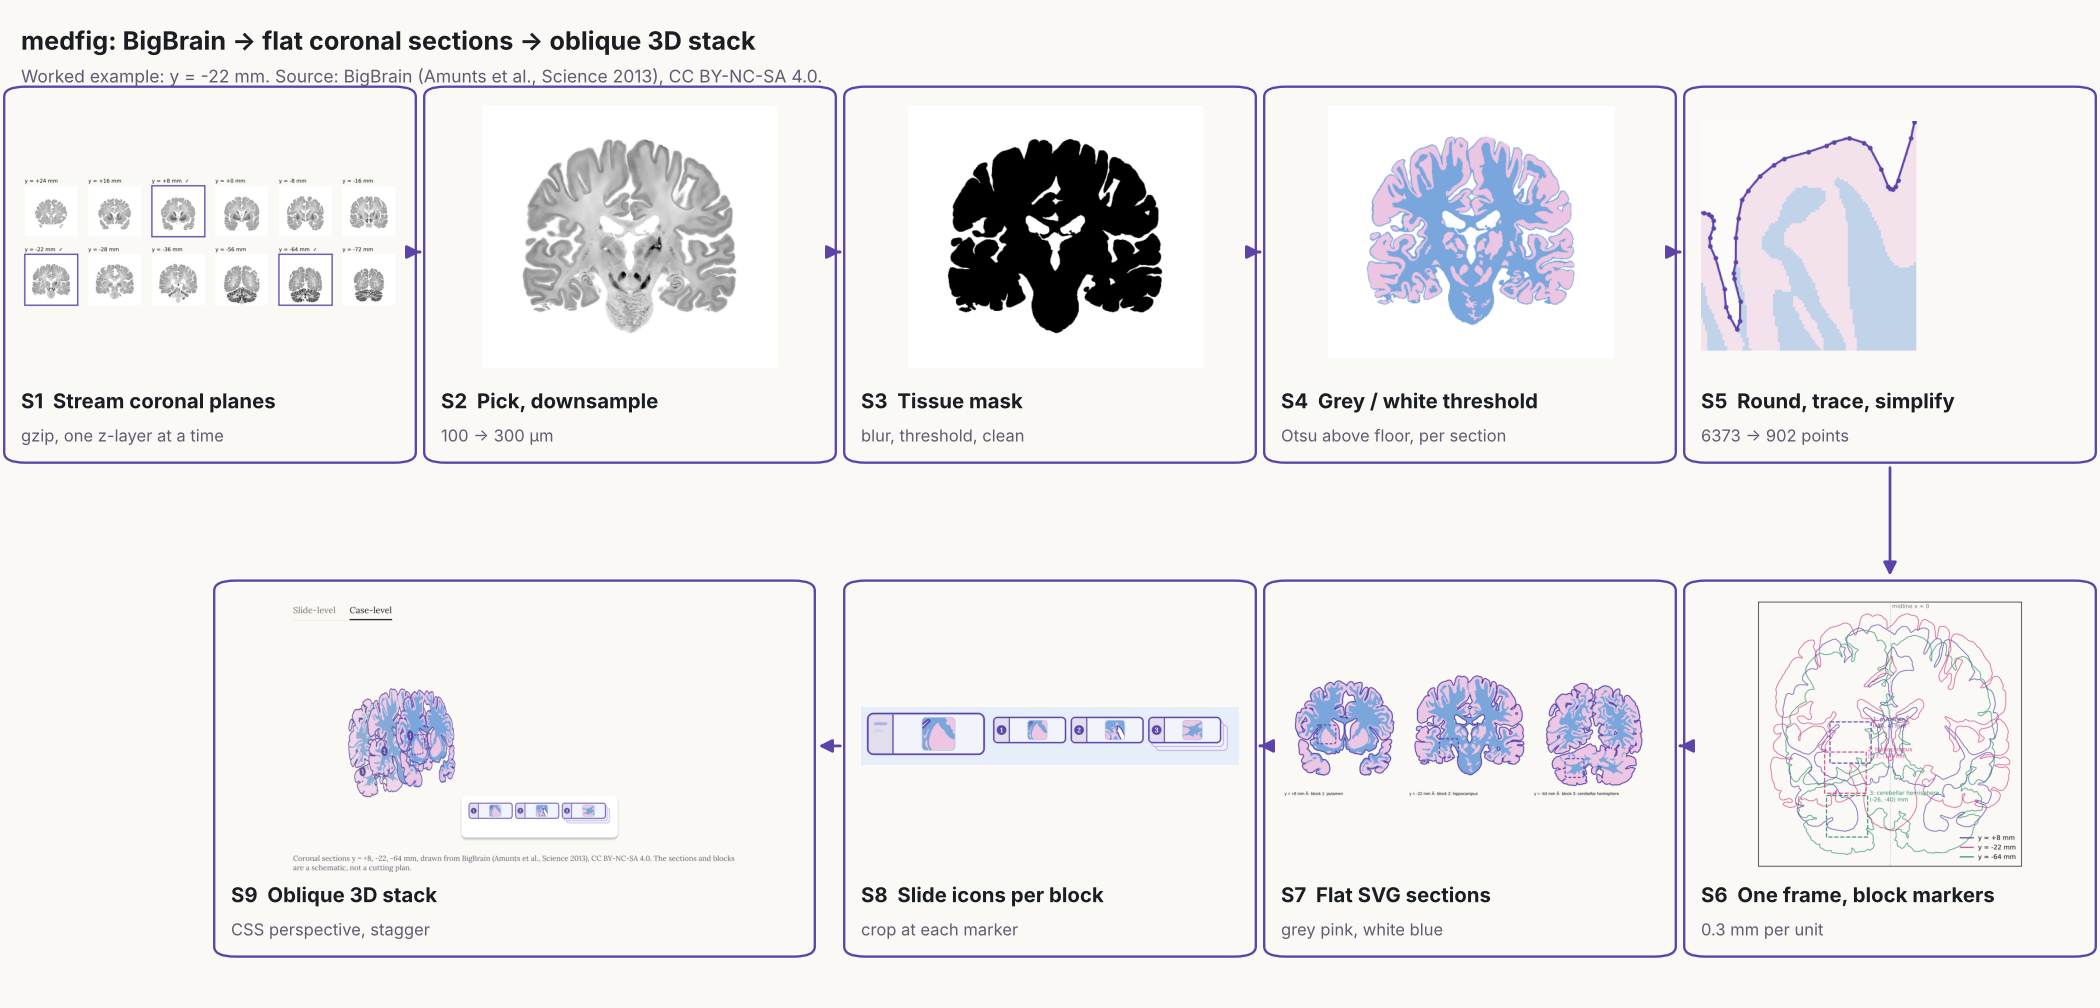
\includegraphics[width=\linewidth]{pipeline_overview.png}
\caption{The nine steps. S1 runs once on the full volume; S2--S9 run from the planes file in seconds. Worked example: $y=\vExampleY$~mm.}
\label{f:overview}
\end{figure}

\begin{table}[H]\centering\small
\begin{tabularx}{\linewidth}{@{}l l X l@{}}\toprule
Step & Module & What it does & Output\\\midrule
S1 & \code{extract} & stream coronal planes out of the volume & \code{data/*.npz}\\
S2 & \code{sections.plane} & flip, block-mean downsample & raster\\
S3 & \code{sections.tissue\_mask} & tissue mask & raster\\
S4 & \code{sections.grey\_white} & per-section grey/white threshold & raster\\
S5 & \code{sections.round\_masks}, \code{smooth\_contour} & round masks, trace, smooth, simplify outlines & polygons\\
S6 & \code{sections.build} & one frame for all sections; block markers & \code{out/sections.json}\\
S7 & \code{sections.build} & SVG drawing & \code{out/section\_k.svg}\\
S8 & \code{icons} & slide icons cut at each block & \code{out/slide\_*.svg}\\
S9 & \code{web}, \code{render} & oblique 3D stack page, frames, end states & \code{out/stack.html}, \code{build/}\\\bottomrule
\end{tabularx}
\caption{Steps, modules and outputs. Run all with \code{make all}.}
\end{table}

\section{Methods}

\subsection{S1 --- Streaming coronal planes}\label{s:s1}
A NIfTI-1 file stores voxels with $x$ varying fastest, then $y$, then $z$. A coronal plane (fixed $y$) is therefore one row in each
of the $n_z$ $z$-layers, spread across the whole file. Because gzip has no random access, \code{extract} decompresses the file
once, layer by layer, and keeps the requested rows. With the sform row $y = s_{y,1}\,j + s_{y,3}$, the voxel index of a plane at
$y$~mm is
\begin{equation}
j(y) = \operatorname{round}\!\left(\frac{y - s_{y,3}}{s_{y,1}}\right).
\end{equation}
Memory is one layer ($n_x n_y = 4.6$~MB) plus the output, below 100~MB; the run time is one pass of gzip over the file
(22~s on the lab PC). Only \code{numpy} is needed.
\begin{figure}[H]\centering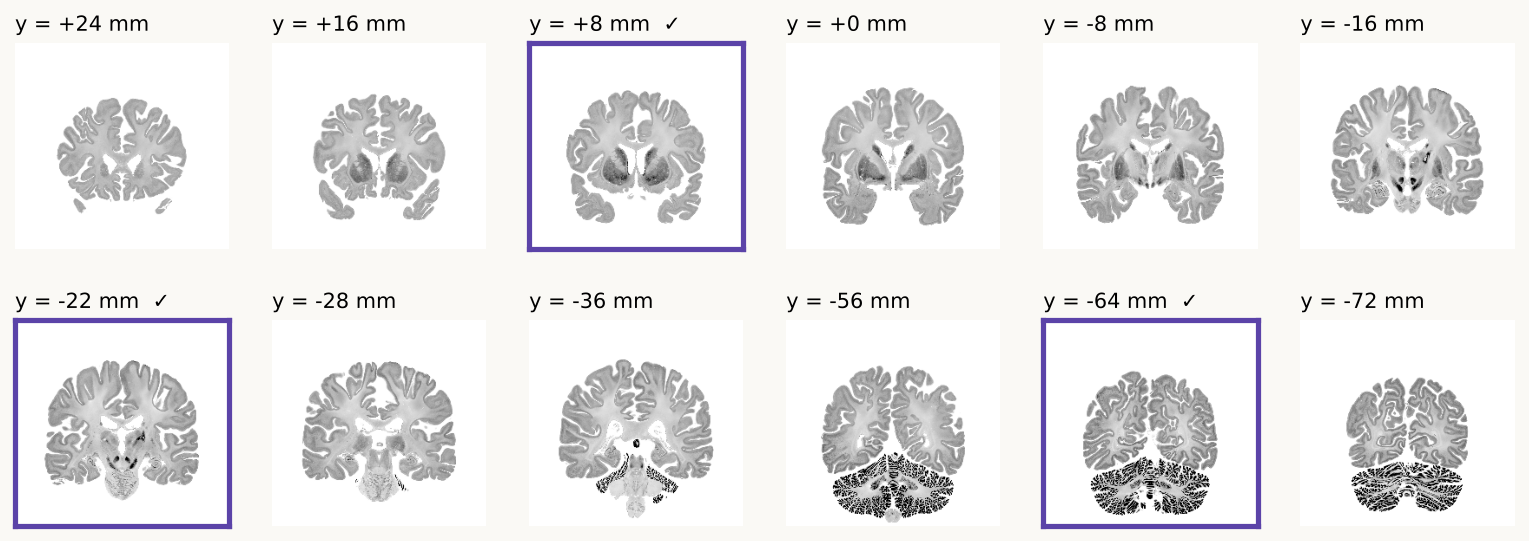
\includegraphics[width=\linewidth]{step_1_candidates.png}
\caption{S1: the \vNPlanes{} candidate planes. The three planes used are framed: $y=+8$ (striatum), $-22$ (thalamus, hippocampus),
$-64$~mm (occipital lobe, cerebellum).}\end{figure}

\subsection{S2 --- Orientation and downsampling}
Each plane is flipped so that rows run superior to inferior, then reduced by a $D\times D$ block mean ($D=\vDs$):
\begin{equation}
a_{ij} = \frac{1}{D^2}\sum_{u=0}^{D-1}\sum_{v=0}^{D-1} I_{Di+u,\;Dj+v},
\end{equation}
from $\vRawW\times\vRawH$ to $\vDownW\times\vDownH$ pixels, $\SI{100}{\micro\metre}\to\SI{300}{\micro\metre}$.
On the page the section is drawn about 250~px wide (about 0.55~px per unit), so detail finer than 0.3~mm is not visible anyway.
\begin{figure}[H]\centering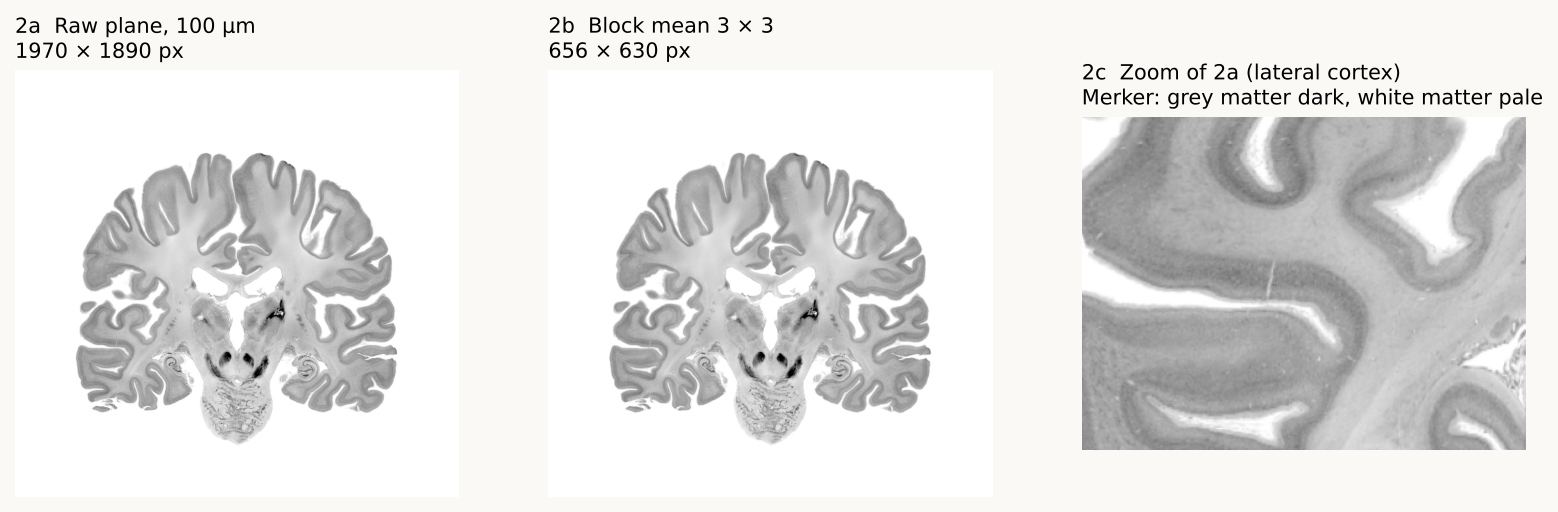
\includegraphics[width=\linewidth]{step_2_plane.png}
\caption{S2 on the worked example.}\end{figure}

\subsection{S3 --- Tissue mask}
With $G_\sigma$ a Gaussian of standard deviation $\sigma$ (pixels),
\begin{equation}
T_0 = \big[\,G_{\vTBlur} * a < \vTMax\,\big],
\end{equation}
then connected components smaller than \vTObj{} px are removed, holes smaller than \vTHole{} px are filled, and one binary opening
smooths the edge. The hole limit is small on purpose: the ventricles and the large sulci stay open. On the worked example, the
cleaning changes \vTissueChanged{} pixels.
\begin{figure}[H]\centering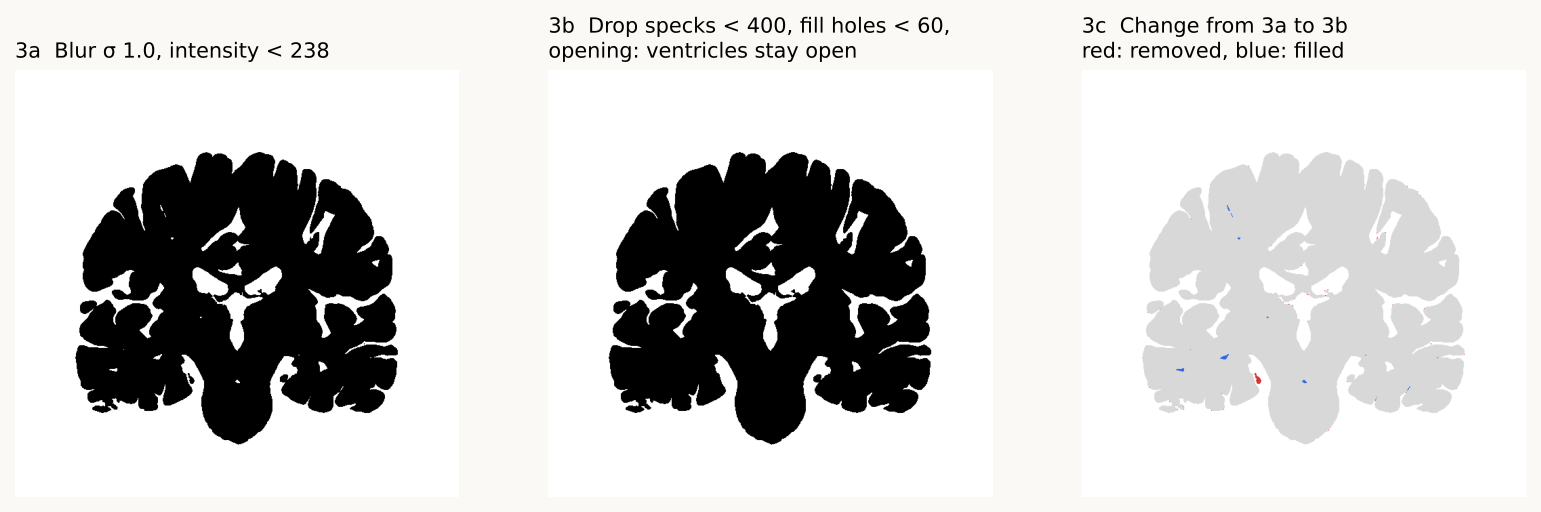
\includegraphics[width=\linewidth]{step_3_tissue.png}
\caption{S3: raw threshold, cleaned mask, and the difference.}\end{figure}

\subsection{S4 --- Grey/white separation}
\paragraph{Local mean.} Intensity is averaged inside the tissue only (normalised convolution), so glass does not brighten the cortex
at the edge:
\begin{equation}
s = \frac{G_{\vLSig} * (a\,T)}{G_{\vLSig} * T}.
\end{equation}
\paragraph{Threshold.} Otsu's method \cite{otsu1979} picks the threshold $t^\ast$ that maximises the between-class variance of a
histogram,
\begin{equation}
t^\ast = \arg\max_t\; \omega_0(t)\,\omega_1(t)\,\big[\mu_0(t)-\mu_1(t)\big]^2,
\end{equation}
where $\omega_{0,1}$ are the class weights and $\mu_{0,1}$ the class means. medfig applies it per section, and only to values above
a floor $f=\vFloor$, then subtracts a small offset $\delta=\vOffset$:
\begin{equation}
t = \operatorname{Otsu}\{\,s_p : p\in T,\ s_p > f\,\} - \delta,\qquad
\mathrm{WM} = T \wedge (s > t).
\end{equation}
The \textbf{floor} matters for the cerebellar section: the granular layer is nearly black and forms a third class, which pulls
Otsu down to about 138 and turns the whole cerebrum into ``white matter'' (Figure~\ref{f:nofloor}, Table~\ref{t:thr}).
A \textbf{per-section} threshold is needed because the stain intensity differs between planes. The offset was chosen by eye
(values 4 and 8 were compared); it makes the cortical ribbon slightly thinner and closer to its real width.

\begin{figure}[H]\centering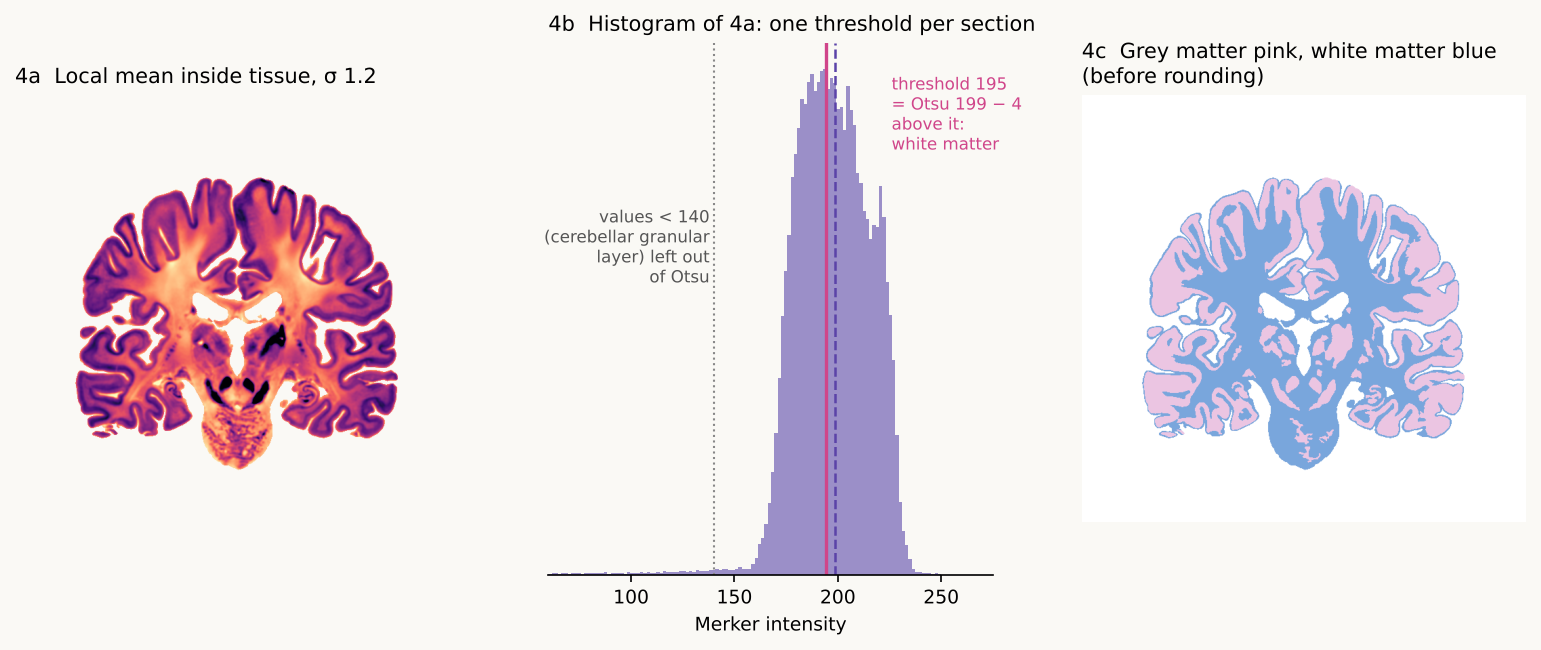
\includegraphics[width=\linewidth]{step_4_grey_white.png}
\caption{S4 on the worked example: local mean, histogram with Otsu ($\vExOtsu$, dashed) and threshold ($\vExThr$, solid),
and the two classes before rounding.}\end{figure}
\begin{figure}[H]\centering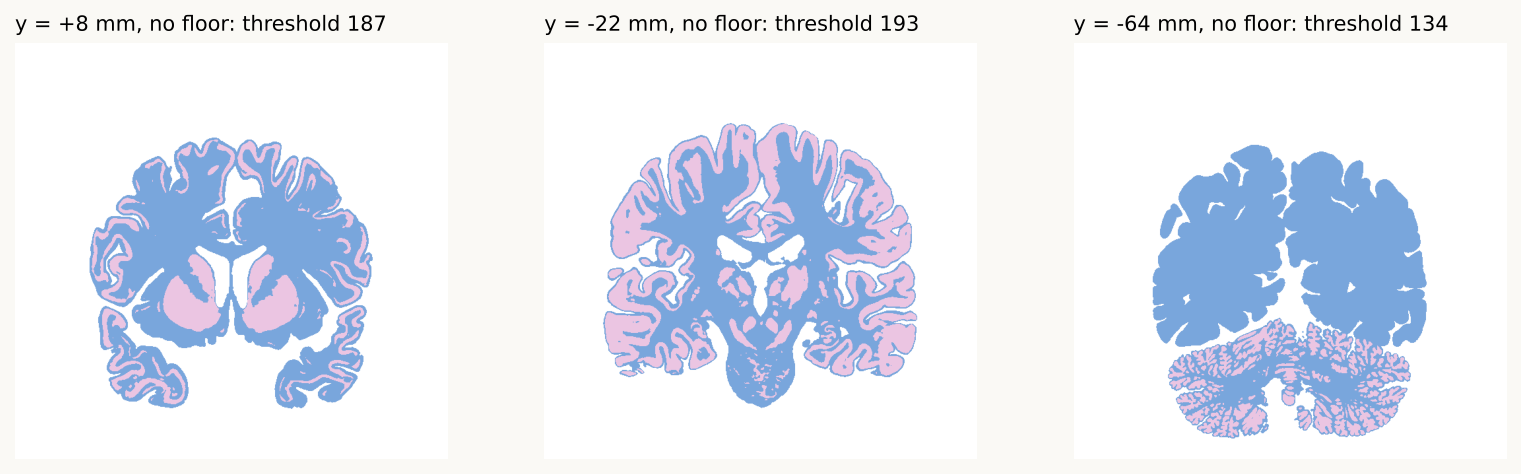
\includegraphics[width=\linewidth]{step_4d_no_floor.png}
\caption{S4 without the floor: on $y=-64$~mm the threshold falls to about 134 and the cerebrum is all blue.}\label{f:nofloor}\end{figure}

\begin{table}[H]\centering\small
\begin{tabularx}{\linewidth}{@{}c r >{\raggedright\arraybackslash}X >{\raggedright\arraybackslash}p{2.3cm} c r r r@{}}\toprule
$k$ & $y$ & Section & Block & Centre $(x,z)$ & Otsu, all & Otsu, $s>f$ & $t$\\\midrule
\SectionRows
\bottomrule\end{tabularx}
\caption{Sections, block positions and thresholds. $y$ and block centres are in MNI millimetres; $x<0$ is drawn on the left of the image.}
\label{t:thr}\end{table}

\subsection{S5 --- Rounding, tracing and simplifying}
Each mask $M$ is blurred and cut at one half, which rounds pixel corners and closes one-pixel gaps:
\begin{equation}
M' = \big[\,G_{\vRSig} * M > 0.5\,\big],
\end{equation}
and white-matter islands smaller than \vWIsl{} px are dropped. Outlines are traced at level 0.5 by marching squares
\cite{lorensen1987,vanderwalt2014} on the mask padded by one pixel (so contours at the image edge close). Each closed contour
$\{(x_n,y_n)\}_{n=0}^{N-1}$ is smoothed with a circular Gaussian,
\begin{equation}
\tilde x_n = \sum_{m} g_m\, x_{(n-m)\bmod N},\qquad g_m \propto e^{-m^2/2\sigma_c^2},\quad \sigma_c=\vCSig,
\end{equation}
and simplified with the Douglas--Peucker algorithm \cite{douglas1973} at tolerance $\varepsilon=\vEps$ units. On the worked example,
all tissue contours go from \vPtsRaw{} to \vPtsSimple{} vertices.
\begin{figure}[H]\centering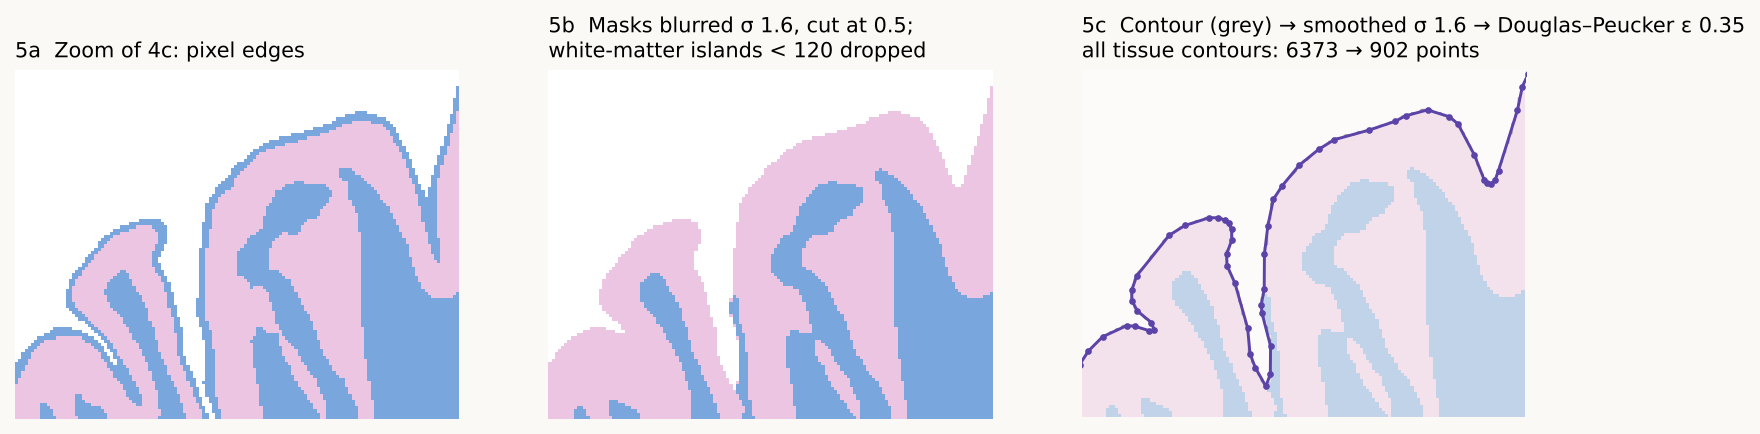
\includegraphics[width=\linewidth]{step_5_contours.png}
\caption{S5, zoom on the dorsal cortex: pixel masks, rounded masks, and the traced (grey), smoothed and simplified (purple) outline.}\end{figure}

\subsection{S6 --- One frame and block markers}
All sections use one scale ($\vMmPerUnit$~mm per unit) and one frame: the bounding box of the union of the tissue masks, padded
by \vPad{} units, gives a $\vVbW\times\vVbH$ viewBox. The midline and $z=0$ fall at the same place in every section, so relative
sizes are real (the $y=-22$~mm section is the widest). A block centre $(x,z)$ in millimetres maps to viewBox units by
\begin{equation}
u = \frac{x - x_0}{\Delta} - o_x,\qquad v = \frac{z_{\mathrm{top}} - z}{\Delta} - o_y,
\end{equation}
with $x_0$ the $x$ of column 0, $z_{\mathrm{top}}$ the $z$ of row 0 after the flip, $\Delta$ the unit size, and $(o_x,o_y)$ the frame
origin. The marker is a \vBlk{}-unit square (about 25~mm) centred on $(u,v)$.
\begin{figure}[H]\centering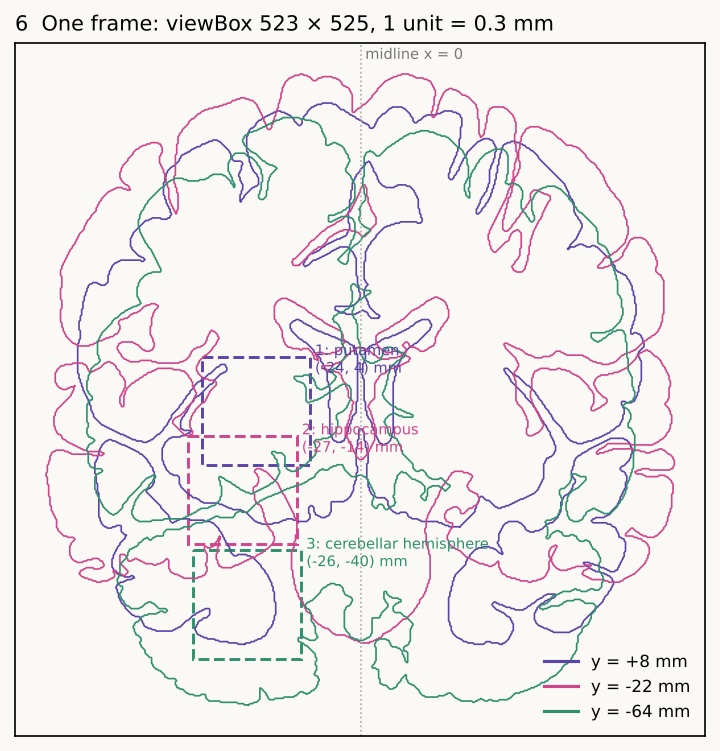
\includegraphics[width=.62\linewidth]{step_6_frame.png}
\caption{S6: the three outlines in the shared frame, with the midline and the three block markers.}\end{figure}

\subsection{S7 --- SVG drawing}
Each section is one SVG with three paths: grey matter (\colorbox{gm}{\strut\ \#ECC6E3\ }, even-odd fill so ventricles stay open),
white matter (\colorbox{wm}{\strut\ \#7AA6DC\ }), and the outline (\textcolor{accent}{\#5B43A8}, width 4.4 units).
Sizes: \SvgSizes.
\begin{figure}[H]\centering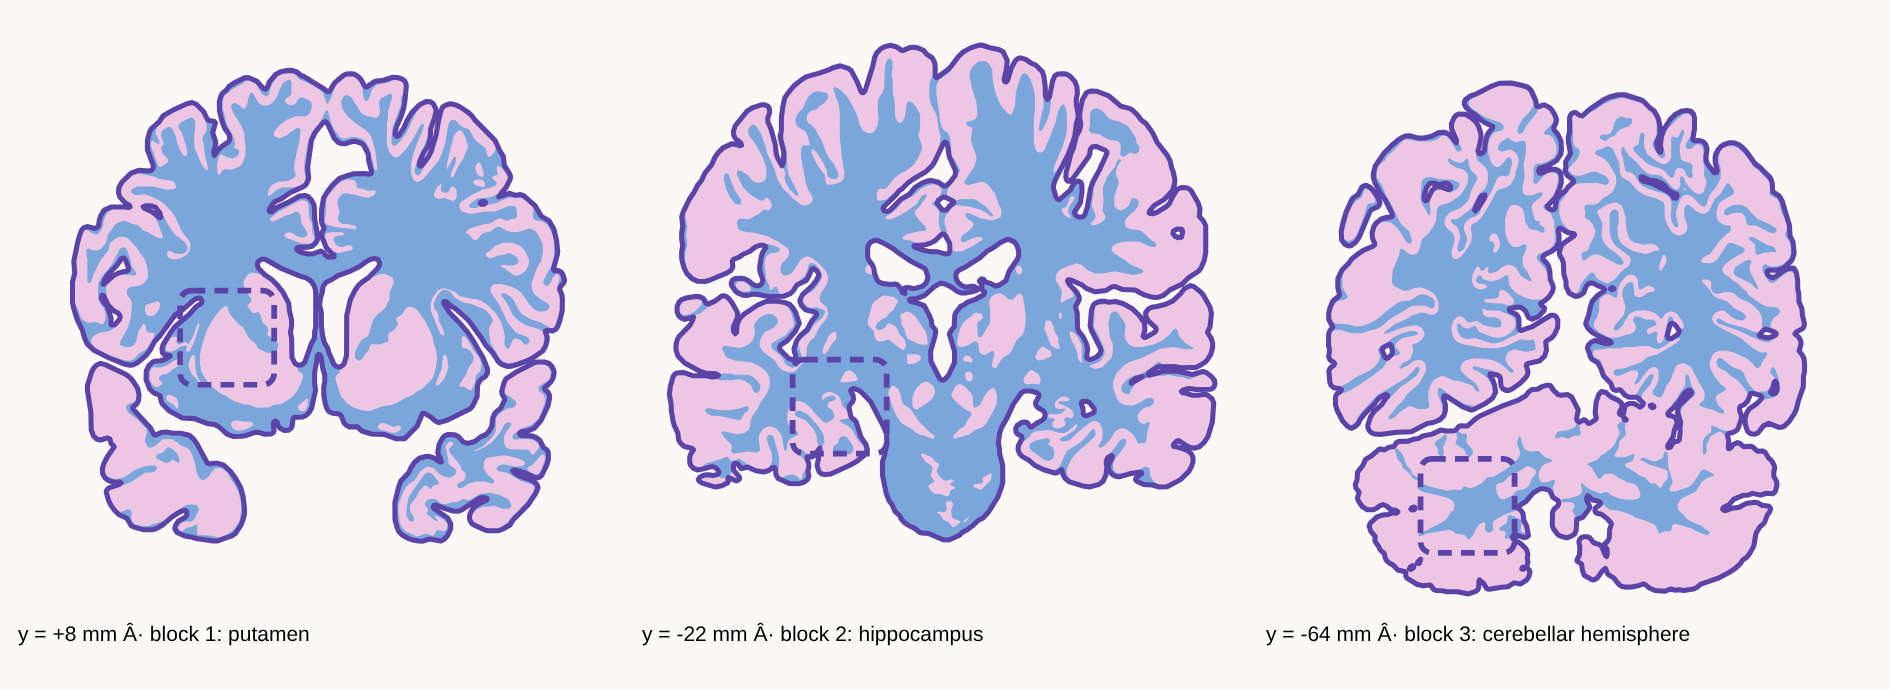
\includegraphics[width=\linewidth]{step_7_svgs.png}
\caption{S7: the three SVG sections with their block markers.}\end{figure}

\subsection{S8 --- Slide icons}
The chat card of the page shows attached slides. Slide $k$ shows section $k$ through an inner \code{<svg>} whose
\code{viewBox} is the block-$k$ rectangle, clipped to a rounded square. Slide and block therefore always match: putamen,
hippocampus, cerebellum.
\begin{figure}[H]\centering
\includegraphics[width=\linewidth]{step_8_icons.png}
\caption{S8: one slide (slide level) and the strip of three slides with the deck behind (case level).}\end{figure}

\subsection{S9 --- Oblique 3D stack}
The stack is plain CSS, so the switch back to slide level is the same motion reversed. The container has perspective
$d=\vPersp$~px. The section stack gets the transform
\begin{equation}
\mathbf{M} = \mathrm{T}_x(\vTx)\;\mathrm{R}_y(\vRy^\circ)\;\mathrm{R}_x(\vRx^\circ)\;\mathrm{S}(\vSc),
\end{equation}
and section $k$ sits at depth $z_k = -\vDz\,(k-1)$~px inside it. A point at depth $z$ (towards the viewer positive) is projected
with scale factor $d/(d-z)$, so the back sections look smaller and fan out to the left. At slide level the back sections wait at
$z=\vZStart$~px with opacity 0. On the switch, the stack turns first, then the back sections slide forward one after the other,
then each block marker appears (Table~\ref{t:timing}). Below \vPhMax~px width the values change to $\mathrm{T}_x(\vPhTx)$,
$\mathrm{R}_y(\vPhRy^\circ)$, $\mathrm{S}(\vPhSc)$, depth step \vPhDz~px. \code{prefers-reduced-motion} turns all motion off.

\begin{table}[H]\centering\small
\begin{tabular}{@{}l c c c@{}}\toprule
 & Section 1 & Section 2 & Section 3\\\midrule
Section starts to move (s) & \SectionDelays\\
Block marker appears (s) & \MarkerDelays\\\bottomrule
\end{tabular}
\caption{Timing after a switch to case level. The stack turn takes 0.75~s, each section 0.7~s.}\label{t:timing}\end{table}

\begin{figure}[H]\centering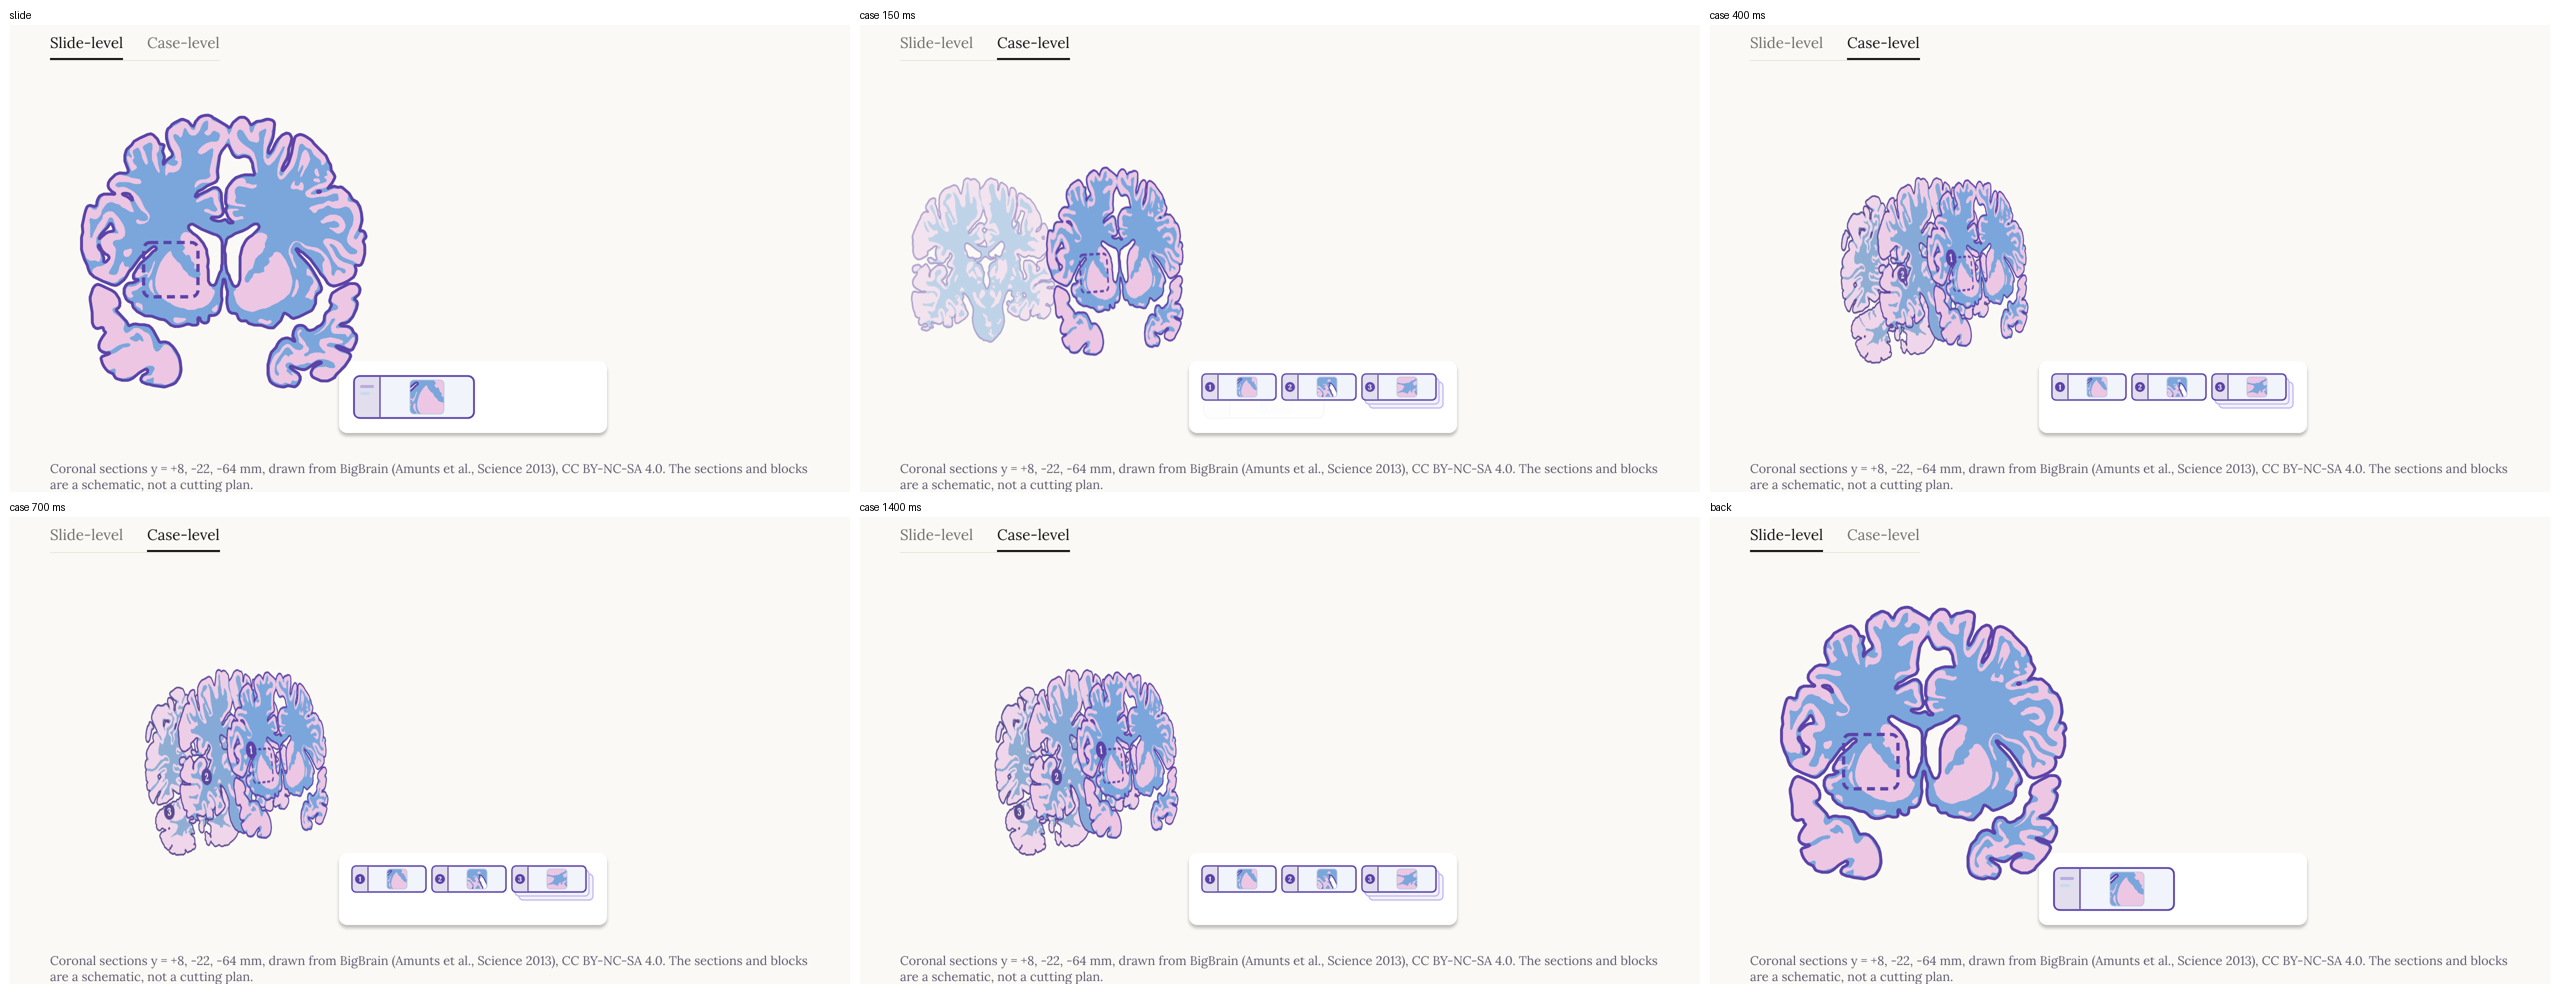
\includegraphics[width=\linewidth]{frame_sheet.png}
\caption{S9: slide level, case level at 150, 400, 700 and 1400~ms, and back to slide level (\code{out/stack.html}, 900~px wide).}\end{figure}

\section{Parameters}
All parameters are in \code{config/sections.json}; \code{MEDFIG\_CONFIG} points to another file. The main ones:

\begin{table}[H]\centering\small
\begin{tabular}{@{}l l r l@{}}\toprule
Step & Key & Value & Effect\\\midrule
S2 & \code{downsample} & \vDs & \SI{100}{\micro\metre} $\to$ \SI{300}{\micro\metre}\\
S3 & \code{tissue\_blur\_sigma}, \code{tissue\_max\_intensity} & \vTBlur, \vTMax & tissue / glass split\\
S3 & \code{tissue\_min\_object\_px}, \code{tissue\_max\_hole\_px} & \vTObj, \vTHole & specks out, ventricles open\\
S4 & \code{local\_mean\_sigma} & \vLSig & smoothing of the grey/white signal\\
S4 & \code{otsu\_floor}, \code{wm\_offset} & \vFloor, \vOffset & granular layer out; ribbon width\\
S5 & \code{mask\_round\_sigma}, \code{wm\_min\_island\_px} & \vRSig, \vWIsl & roundness; fewer specks\\
S5 & \code{contour\_sigma}, \code{dp\_epsilon} & \vCSig, \vEps & outline smoothness; vertex count\\
S6 & \code{pad\_units}, \code{block\_units} & \vPad, \vBlk & frame margin; marker size\\
S9 & \code{case.rotate\_y\_deg}, \code{case.depth\_step\_px} & \vRy, \vDz & fan angle; gap between sections\\\bottomrule
\end{tabular}\end{table}

\paragraph{Other planes or blocks.} Change \code{sections} (each $y$ must be in the planes file, or run \code{extract} with
\code{--y}). Any number of sections works; the timing lists extend with default steps.

\section{Verification}
\begin{itemize}
\item \code{make test} (pytest, 5 checks): the planes file shape; tissue and white-matter fractions in a sane range for every
section; the floor raises the cerebellar Otsu by more than 20; two builds give byte-identical SVGs and every marker is inside the
frame; the SVG path data equal the copies published on the lab landing page on 13 October 2026 (\code{tests/reference/}).
\item \code{medfig render} reports the page width at 900 and 390~px (no horizontal scroll) and page errors (none).
\item The figures in this report are made by the same functions as the products (\code{medfig/figures.py}).
\end{itemize}

\section{Reproduction and DGX Spark}
\begin{lstlisting}
git clone medfig.bundle medfig && cd medfig
scripts/dgx_setup.sh            # venv, pip install, Chromium, checksum, tests
. .venv/bin/activate
make all                        # sections, icons, web, figures, render, overview, report
make extract VOLUME=/path/full8_100um_2009b_sym.nii.gz   # only to cut new planes
\end{lstlisting}
\paragraph{Notes for DGX Spark.} DGX Spark is an aarch64 machine. As far as we know, all Python dependencies have aarch64 wheels and Playwright ships
Chromium for linux-arm64. Neither statement has been checked on a DGX Spark yet; \code{scripts/dgx\_setup.sh} is the first test. The pipeline uses the CPU only: S2--S7 take a few seconds, S1 is limited by gzip (one core). If S1 has to run
often, a parallel gzip reader (for example \code{rapidgzip}) or an uncompressed copy of the volume will make it I/O-bound. The GPU is
not needed; it becomes useful only for heavier future steps, for example 3D surface extraction from the full volume.

\section{Limitations}
\begin{enumerate}
\item \textbf{Schematic.} One brain, three planes, blocks chosen for illustration. Not the BU cutting plan, not BU block locations.
\item \textbf{Block centres} were set from general MNI anatomy, not from an atlas lookup. Check them against an atlas
(for example Harvard--Oxford) before any figure that claims a structure.
\item \textbf{Stain.} BigBrain is Merker-stained. The pink/blue colouring is a drawing convention, not a stain simulation.
\item \textbf{Threshold.} The grey/white split is a global intensity rule per section. It does not follow cortical layers, and
deep nuclei are drawn as grey matter.
\item \textbf{Phones.} At 390~px the three sections are about 70~px wide each and look crowded.
\end{enumerate}

\section{Licence and credits}
Data: BigBrain \cite{amunts2013}, CC BY-NC-SA 4.0. Every derived figure in \code{out/} and \code{build/} is adapted material under
CC BY-NC-SA 4.0 and must carry the credit line
``Brain sections drawn from BigBrain (Amunts et al., Science 2013), CC BY-NC-SA 4.0''. Software: NumPy, SciPy, scikit-image
\cite{vanderwalt2014}, Matplotlib, Pillow, Playwright.

\begin{thebibliography}{9}\small
\bibitem{amunts2013} K.~Amunts et al. BigBrain: an ultrahigh-resolution 3D human brain model. \emph{Science} 340(6139):1472--1475, 2013.
\bibitem{fonov2011} V.~Fonov et al. Unbiased average age-appropriate atlases for pediatric studies. \emph{NeuroImage} 54(1):313--327, 2011.
\bibitem{otsu1979} N.~Otsu. A threshold selection method from gray-level histograms. \emph{IEEE Trans.\ Systems, Man, and Cybernetics} 9(1):62--66, 1979.
\bibitem{lorensen1987} W.~E.~Lorensen and H.~E.~Cline. Marching cubes: a high resolution 3D surface construction algorithm. \emph{SIGGRAPH} 21(4):163--169, 1987.
\bibitem{douglas1973} D.~H.~Douglas and T.~K.~Peucker. Algorithms for the reduction of the number of points required to represent a digitized line or its caricature. \emph{Cartographica} 10(2):112--122, 1973.
\bibitem{vanderwalt2014} S.~van der Walt et al. scikit-image: image processing in Python. \emph{PeerJ} 2:e453, 2014.
\end{thebibliography}

\appendix
\section{Repository map}
\begin{lstlisting}
config/sections.json      every parameter
data/                     planes file (10 MB), checksum, licence note
medfig/extract.py         S1   stream planes from the .nii.gz
medfig/sections.py        S2-S7 rasters -> vector SVG, shared frame, markers
medfig/icons.py           S8   slide icons
medfig/web.py             S9   stack page, CSS, markup snippet
medfig/render.py          S9   frames, frame sheet, end states, GIF, figures S7-S8
medfig/figures.py         report figures S1-S6 and numbers.json
medfig/overview.py        Figure 1
medfig/report.py          report/numbers.tex
medfig/site_export.py     copy products into a host site
tests/                    checks and reference SVGs
report/report.tex         this report
scripts/dgx_setup.sh      environment setup
\end{lstlisting}
\end{document}
